\documentclass[10pt,twocolumn]{article}
\usepackage[margin=0.75in]{geometry}
\usepackage{times}
\usepackage{graphicx}
\usepackage{subcaption}
\usepackage{amsmath}
\usepackage{amssymb}
\usepackage[numbers]{natbib}
\usepackage[bookmarks=true]{hyperref}
\usepackage{tikz}
\usetikzlibrary{arrows.meta, positioning, shapes.geometric}

\begin{document}

\title{\Large\bfseries Posterior-Guided Domain Randomization via Sampling-Based System Identification for Humanoid Locomotion}

\author{
{Mohammad Al Masalmeh \quad Andrew Liu \quad Krish Patel-Shah \quad Mario Perales III \quad Angel Lemus} \\
\textit{Department of Computer Science, The University of Texas at Austin}
}
\maketitle

\begin{abstract}
Sim-to-real transfer for humanoid locomotion faces a fundamental tension: domain randomization (DR) provides robustness but sacrifices precision, while system identification (sys-id) provides precision but is brittle to unmodeled effects.
We propose \textbf{Posterior-Guided Domain Randomization} (PGDR), a method that resolves this tension by treating sys-id not as a way to find a single best parameter setting, but as a way to learn \emph{where the uncertainty lies} in the parameter space.
The key observation is simple: when a sampling-based optimizer like CMA-ES converges on physical parameters that match real-world data, it also reveals which parameters it could pin down confidently and which remained ambiguous.
Parameters that are ambiguous after identification are exactly the ones a policy should be robust to.
Concretely, we run CMA-ES over massively parallel MuJoCo MJX rollouts of the Booster T1 humanoid to recover both a point estimate $p^*$ and the optimizer's final covariance $\Sigma$, then train locomotion policies under a Gaussian DR distribution $\mathcal{N}(p^*, \alpha\Sigma)$.
This distribution is tight along well-identified parameter directions and wide along uncertain ones, providing targeted robustness at zero additional computational cost since CMA-ES already maintains the covariance as part of its search.
We validate on the Booster T1 humanoid via sim-to-sim experiments with known ground truth and zero-shot sim-to-real deployment, comparing against uniform DR, pure sys-id, and isotropic narrow DR on joystick velocity tracking.
\end{abstract}

% ====================================================================
\section{Introduction}
% ====================================================================

Reinforcement learning can produce agile locomotion in simulation, but deploying these policies on physical humanoid robots remains difficult due to the sim-to-real gap: the mismatch between simulated and real-world dynamics.
The field's response to this problem has progressed through a chain of solutions, each fixing a limitation of the previous one but leaving a remaining weakness.
We identify and close the gap left by the most recent link in this chain.

\subsection{The Chain of Solutions}

\textbf{Problem 1: The sim-to-real gap.}
Simulated physics never perfectly match the real world, so policies trained in simulation often fail on hardware.
\emph{Domain randomization} (DR)~\cite{peng2018sim2real} addresses this by training policies across broad distributions of physical parameters (mass, friction, actuator gains), producing behaviors robust to any particular dynamics setting.
This is the default strategy in most sim-to-real pipelines, including MuJoCo Playground's Booster T1 environment~\cite{zakka2025playground}.

\textbf{Problem 2: DR requires manual tuning and produces conservative policies.}
Broad randomization forces the policy to handle \emph{every} possible dynamics setting, preventing it from exploiting the specific structure of the \emph{actual} system.
Practitioners must hand-tune randomization ranges: too wide and the policy is overly conservative, too narrow and the real parameters fall outside the training distribution.
\emph{System identification} (sys-id) addresses this by estimating the real robot's physical parameters directly, so the simulator can be configured to match reality and the policy can train in a precise environment.
SPI-Active~\cite{sobanbabu2025spiactive} makes this practical for legged robots by using CMA-ES over massively parallel GPU simulations to find the parameter vector whose rollouts best match observed real-world trajectories.

\textbf{Problem 3: Sys-id point estimates overfit, and SPI-Active still relies on hand-tuned DR.}
This is the problem we solve.
No parameter estimate is perfect: the identified parameters match the specific trajectories used for calibration, but unmodeled effects (actuator thermal drift, cable routing forces, floor variation) mean the real system will never exactly match any single simulation configuration.
A policy trained at the identified point estimate is brittle to these residual mismatches, in the same way that a supervised learning model trained without regularization overfits to its training data.
SPI-Active recognizes this and adds narrow DR around the identified parameters, but the ranges of this narrow DR are hand-tuned by the researchers (Appendix~A.4.3 of~\cite{sobanbabu2025spiactive}).
This reintroduces the same manual tuning problem that motivated moving away from DR in the first place.
SPI-Active's argument is that blind DR is suboptimal because you should identify the real parameters instead, yet the method still falls back on hand-tuned DR after identification.

\subsection{Our Solution}

We observe that the information needed to set DR ranges automatically already exists inside the sys-id optimizer.
CMA-ES works by maintaining a search distribution $\mathcal{N}(\mu_k, \sigma_k^2 C_k)$ over the parameter space and iteratively refining it.
At convergence, the covariance of this search distribution reflects identification uncertainty:

\begin{itemize}
    \item \textbf{Well-identified parameters} (e.g., link masses, actuator gains) produce sharp valleys in the loss landscape. CMA-ES contracts its covariance tightly along these directions because deviating from the optimum causes large increases in trajectory mismatch. These parameters are pinned down by the data; the policy can safely specialize to the identified values.
    \item \textbf{Poorly-identified parameters} (e.g., ground contact properties, joint friction coefficients) produce flat regions in the loss landscape. Many different values produce similar trajectories, so CMA-ES cannot contract its covariance along these directions. These are exactly the parameters that pose a sim-to-real risk: if the optimizer cannot distinguish between values, neither can the data, and the true value could be anywhere in that uncertain region. The policy needs robustness here.
\end{itemize}

We propose \textbf{Posterior-Guided Domain Randomization} (PGDR): after sys-id converges, retain the optimizer's final covariance $\Sigma$ alongside the point estimate $p^*$, and train the downstream locomotion policy with parameters sampled from $\mathcal{N}(p^*, \alpha\Sigma)$ at each training episode.

This replaces SPI-Active's hand-tuned narrow DR with a data-driven distribution that is automatically tight along well-identified directions and wide along uncertain ones.
The approach costs nothing extra (CMA-ES already computes and maintains the covariance as part of its search) and eliminates manual range tuning entirely.

\subsection{Contributions}

\begin{enumerate}
    \item \textbf{PGDR}: A method that unifies sys-id and DR by repurposing the CMA-ES covariance from parameter identification as the DR distribution for policy training.
    The key insight is that the information needed to set principled DR ranges is a free byproduct of sampling-based sys-id: parameters the optimizer could not pin down are precisely the ones the policy should be robust to.
    \item \textbf{Controlled ablations} isolating the value of anisotropic uncertainty: we compare PGDR against pure sys-id ($\alpha=0$), isotropic narrow DR (same center, same total spread, but uniform in all directions), and standard uniform DR on both nominal and perturbed conditions.
    \item \textbf{Booster T1 deployment}: We implement the full pipeline on the Booster T1 humanoid using MuJoCo Playground's MJX backend, providing an independent validation of sampling-based sys-id on a platform and simulator not previously studied (SPI-Active uses Unitree robots on IsaacGym).
\end{enumerate}

% ====================================================================
\section{Related Work}
% ====================================================================

\subsection{Sampling-Based System Identification}

Sobanbabu~et~al.~\cite{sobanbabu2025spiactive} introduce SPI-Active, a two-stage framework and the closest prior work to ours.
Stage~1 collects real-world trajectories using pre-trained RL policies, then estimates physical parameters by minimizing state prediction error between simulated and real rollouts via CMA-ES over massively parallel GPU simulations.
Stage~2 introduces active exploration: it optimizes velocity commands to maximize the Fisher Information of collected trajectories, improving identification of under-excited parameters.
SPI-Active achieves 42--63\% improvement over DR baselines on the Unitree Go2 quadruped and G1 humanoid.

Our method builds directly on SPI-Active's Stage~1.
The critical difference is what happens \emph{after} identification.
SPI-Active trains policies at the identified point estimate with hand-tuned narrow DR around it (Appendix~A.4.3 of~\cite{sobanbabu2025spiactive}), treating the covariance as a search artifact to be discarded.
We instead treat the covariance as the deliverable: it encodes exactly which parameters were well-constrained by the data and which were not, and we use this to shape the training distribution automatically.
We also port the pipeline from IsaacGym to MuJoCo MJX and evaluate on the Booster T1 rather than Unitree platforms.

\subsection{Domain Randomization}

Peng~et~al.~\cite{peng2018sim2real} establish dynamics randomization as the standard sim-to-real paradigm by varying mass, friction, and damping during training.
Rudin~et~al.~\cite{rudin2022learning} demonstrate that DR combined with GPU-parallel simulation enables humanoid walking training in minutes.
The fundamental limitation of all DR approaches is that randomization ranges must be specified manually.
Too wide and the policy becomes conservative; too narrow and the real parameters may fall outside the training distribution.
PGDR replaces this manual specification with ranges derived directly from identification data.

\subsection{Rapid Motor Adaptation}

Kumar~et~al.~\cite{kumar2021rma} pair a base policy with an online adaptation module that estimates latent extrinsic parameters from proprioceptive history at deployment time.
RMA addresses a complementary problem: it handles \emph{runtime} variation (a robot stepping onto a new surface mid-episode), whereas PGDR addresses \emph{training-time} calibration (ensuring the training distribution matches the real system).
The two could be composed: PGDR to set the training distribution, RMA to handle residual mismatch at deployment.

\subsection{Cross-Simulator Dynamics Alignment}

He~et~al.~\cite{he2025asap} propose ASAP, which learns a delta-action residual correction at deployment time to align simulator and real-world physics.
Like RMA, this is a deployment-time correction complementary to our training-time approach.

\subsection{Adaptive Environment Generation}

Yu~et~al.~\cite{yu2025adept} propose ADEPT, which uses a diffusion model to generate training terrain configurations at the frontier of a policy's competence.
While ADEPT operates over terrain geometry rather than dynamics parameters, there is a shared principle: both methods replace uniform sampling with structured distributions that concentrate on the most informative regions of the configuration space.

\subsection{Real-World Humanoid Locomotion}

Radosavovic~et~al.~\cite{radosavovic2024humanoid} achieve zero-shot sim-to-real humanoid locomotion via a causal transformer trained on large randomized environment ensembles.
Their reliance on very large ensembles illustrates the cost of using broad DR alone for robustness; our approach instead narrows the distribution to where the uncertainty actually is.

\subsection{Adversarial Robustness Training}

Pinto~et~al.~\cite{pinto2017robust} train policies against an adversary that applies destabilizing perturbations, providing worst-case robustness.
This is orthogonal to PGDR's average-case robustness along uncertain parameter directions.

\subsection{MuJoCo Playground and Booster T1}

Zakka~et~al.~\cite{zakka2025playground} introduce MuJoCo Playground and demonstrate joystick velocity tracking on the Booster T1~\cite{boostert1} using standard uniform DR.
The T1 is a 23-DoF humanoid with onboard NVIDIA AGX Orin compute, five classes of integrated actuators (7--130\,Nm), and a 9-axis IMU.
Its open-source MuJoCo model and MuJoCo Playground's MJX-based training pipeline provide our simulation infrastructure.

% ====================================================================
\section{Method}
% ====================================================================

\subsection{Overview}

The intuition behind PGDR is that system identification produces more than just a best-guess parameter vector: it also reveals the structure of the uncertainty around that guess.
Our pipeline extracts both pieces of information and feeds them into policy training.

The three phases (Figure~\ref{fig:pipeline}):
\begin{enumerate}
    \item \textbf{Data collection}: Collect reference trajectories from the real robot (or a held-out simulator for validation).
    \item \textbf{Identification}: Run CMA-ES over parallel MJX rollouts to find the parameters $p^*$ that best reproduce the reference trajectories.  Retain the optimizer's final covariance $\Sigma$, which encodes identification uncertainty.
    \item \textbf{Policy training}: Train a locomotion policy via RL, sampling physical parameters from $\mathcal{N}(p^*, \alpha\Sigma)$ at each episode.  The policy sees more variation along uncertain parameter directions and less along confident ones.
\end{enumerate}

\begin{figure}[t]
\centering
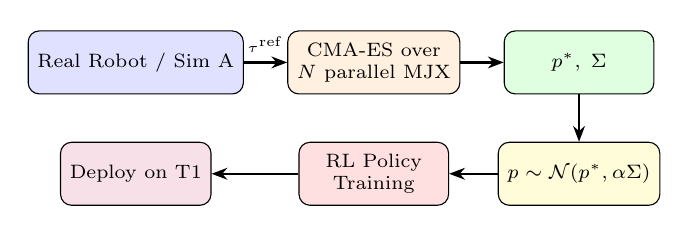
\begin{tikzpicture}[
    node distance=0.45cm and 0.55cm,
    block/.style={rectangle, draw, rounded corners, minimum height=0.8cm, minimum width=1.9cm, align=center, font=\scriptsize},
    arrow/.style={-{Stealth[length=2mm]}, thick},
]
    \node[block, fill=blue!12] (real) {Real Robot / Sim A};
    \node[block, fill=orange!12, right=of real] (cmaes) {CMA-ES over\\$N$ parallel MJX};
    \node[block, fill=green!12, right=of cmaes] (post) {$p^*,\; \Sigma$};
    \node[block, fill=yellow!15, below=0.6cm of post] (dr) {$p \sim \mathcal{N}(p^*, \alpha\Sigma)$};
    \node[block, fill=red!12, below=0.6cm of cmaes] (train) {RL Policy\\Training};
    \node[block, fill=purple!12, below=0.6cm of real] (deploy) {Deploy on T1};

    \draw[arrow] (real) -- node[above, font=\tiny] {$\tau^{\mathrm{ref}}$} (cmaes);
    \draw[arrow] (cmaes) -- (post);
    \draw[arrow] (post) -- (dr);
    \draw[arrow] (dr) -- (train);
    \draw[arrow] (train) -- (deploy);
\end{tikzpicture}
\caption{PGDR pipeline.  CMA-ES identification produces both a point estimate $p^*$ and covariance $\Sigma$.  Policy training samples parameters from the resulting uncertainty-shaped distribution.}
\label{fig:pipeline}
\end{figure}

\subsection{Parameter Identification via CMA-ES}

Let $p \in \mathbb{R}^d$ denote the physical parameter vector (joint friction, link mass offsets, actuator gains, ground contact properties; $d \approx 65$ for the T1).
Given reference trajectories $\tau^{\mathrm{ref}}$ collected under known actions, we seek the parameters that make the simulator best reproduce those trajectories by minimizing:
\begin{equation}
    \mathcal{L}(p) = \frac{1}{T}\sum_{t=1}^{T} \left[ w_q \| q_t^{\mathrm{sim}}(p) - q_t^{\mathrm{ref}} \|^2 + w_{\dot{q}} \| \dot{q}_t^{\mathrm{sim}}(p) - \dot{q}_t^{\mathrm{ref}} \|^2 \right],
    \label{eq:loss}
\end{equation}
where $q_t, \dot{q}_t$ are joint positions and velocities.

CMA-ES is a derivative-free optimizer that searches by maintaining and refining a Gaussian distribution over the parameter space.
At each generation $k$, it:
\begin{enumerate}
    \item Samples $N$ candidate parameter vectors from $\mathcal{N}(\mu_k, \sigma_k^2 C_k)$.
    \item Rolls out all $N$ candidates in parallel via MJX and evaluates $\mathcal{L}(p^{(i)})$.
    \item Updates the mean $\mu_{k+1}$, step size $\sigma_{k+1}$, and covariance $C_{k+1}$ based on the best-performing candidates.
\end{enumerate}

The covariance update is the mechanism that matters for PGDR.
CMA-ES adapts $C_k$ so that its search elongates along directions where different parameter settings produce different loss values (high sensitivity) and stays wide along directions where the loss is relatively flat (low sensitivity).
At convergence (generation $K$), the search distribution has contracted tightly along directions that the data constrains well and remains broad along directions that the data cannot resolve.

We extract both outputs:
\begin{align}
    p^* &= \mu_K, \label{eq:pstar} \\
    \Sigma &= \sigma_K^2 \, C_K. \label{eq:sigma}
\end{align}

Standard practice uses only $p^*$ and discards $\Sigma$.
We retain both.

\subsection{Why the Covariance Encodes Useful Uncertainty}

To build intuition for why $\Sigma$ is informative, consider two types of parameters:

\textbf{A well-identified parameter}, such as the mass of the torso link: changing the torso mass by 5\% produces noticeably different joint trajectories under the same actions, because the torso mass affects the dynamics of every joint.
CMA-ES quickly narrows its search distribution along this direction because candidates with the wrong torso mass perform poorly.
The corresponding eigenvalue in $\Sigma$ is small.

\textbf{A poorly-identified parameter}, such as the coefficient of restitution of the foot-ground contact: moderate changes to restitution have little effect on steady-state walking trajectories, because the foot spends most of its contact phase in sustained contact rather than bouncing.
CMA-ES cannot distinguish between restitution values of, say, 0.1 and 0.3, so its search distribution stays broad in this direction.
The corresponding eigenvalue in $\Sigma$ is large.

The poorly-identified parameter is exactly the one that poses a sim-to-real risk: if the optimizer cannot tell whether restitution is 0.1 or 0.3, the true value could be either, and the policy should be robust to both.
A well-identified parameter, by contrast, is pinned down by the data, so the policy can safely specialize to the identified value.

We note that $\Sigma$ is not a Bayesian posterior in the strict sense; CMA-ES is an optimizer, not a probabilistic inference algorithm.
However, it serves as a practical proxy for identification uncertainty, and we validate this interpretation empirically in our sim-to-sim experiments (Section~\ref{sec:experiments}).

\subsection{Posterior-Guided Domain Randomization}

Given $p^*$ and $\Sigma$, we train the downstream locomotion policy with parameters sampled at each episode from:
\begin{equation}
    p \sim \mathcal{N}(p^*, \; \alpha \Sigma), \quad \alpha > 0.
    \label{eq:pgdr}
\end{equation}

The scalar $\alpha$ controls the overall scale of randomization:
\begin{itemize}
    \item $\alpha = 0$: Pure sys-id.  The policy trains at $p^*$ only, with no randomization.  This gives maximum precision but no robustness to residual mismatch.
    \item Small $\alpha$ (e.g., 0.5--1.0): Tight randomization concentrated around $p^*$, with the spread shaped by identification uncertainty.  This is the regime we expect to work best: the policy exploits the identified dynamics while maintaining robustness where the identification is uncertain.
    \item Large $\alpha$ (e.g., 2.0+): Wider randomization that approaches uniform DR in scale but retains the anisotropic shape.
\end{itemize}

The critical property of PGDR is \emph{anisotropy}.
Standard narrow DR shrinks all randomization ranges by a uniform factor, treating every parameter as equally uncertain.
PGDR instead randomizes each parameter in proportion to how uncertain the identification process was about that parameter.
This means the policy does not waste capacity being robust to variation in parameters that are already well-known, and instead focuses its robustness budget on parameters that genuinely could differ between simulation and reality.

\subsection{Analogy to Regularization in Supervised Learning}

The relationship between pure sys-id and PGDR mirrors the relationship between unregularized and regularized fitting in supervised learning.
A model trained on finite data without regularization overfits to the specific noise realization in the training set.
Similarly, a policy trained at a single identified parameter vector overfits to the specific conditions of the calibration trajectories.
Adding structured noise during training (PGDR) acts as a form of regularization, where the noise structure is informed by the data rather than chosen arbitrarily.

\subsection{Parameter Space for the Booster T1}

We target the following groups, subject to reduction after sensitivity analysis:
\begin{itemize}
    \item \textbf{Joint friction} (23 params): viscous friction per actuated joint.
    \item \textbf{Link mass offsets} ($\sim$15 params): additive corrections to link masses.
    \item \textbf{Actuator gain scaling} (23 params): multiplicative factors on PD targets or commanded torques.
    \item \textbf{Ground contact} (4 params): stiffness, damping, friction, restitution.
\end{itemize}
Total dimension $d \approx 65$.
We expect sensitivity analysis to reveal that many of these are negligible, allowing dimensionality reduction before the final identification run.

% ====================================================================
\section{Experimental Plan}
\label{sec:experiments}
% ====================================================================

Our experiments are designed to answer three questions:
\begin{enumerate}
    \item Does the CMA-ES covariance actually reflect identification uncertainty? (Validated in sim-to-sim where ground truth is known.)
    \item Does shaping noise by this uncertainty (PGDR) outperform uniform noise of the same total magnitude? (The C3 vs.\ C4 ablation.)
    \item Does PGDR transfer to real hardware? (Sim-to-real deployment.)
\end{enumerate}

\subsection{Sim-to-Sim Validation}

We first validate in a controlled setting where ground truth is known:
\begin{enumerate}
    \item Configure \textbf{Sim~A} with a fixed parameter vector $p^{\mathrm{true}}$ that deviates from the MuJoCo default model (e.g., 10--20\% perturbations to mass, friction, actuator gains).
    \item Run identification from \textbf{Sim~B} using Sim~A trajectories as reference, obtaining $p^*$ and $\Sigma$.
    \item Verify that $\Sigma$ is informative: parameters where $p^*$ deviates most from $p^{\mathrm{true}}$ should correspond to large eigenvalues in $\Sigma$ (the optimizer was uncertain about them), while well-recovered parameters should correspond to small eigenvalues.
    \item Train policies under all four conditions (below) and evaluate in Sim~A.
\end{enumerate}

This controlled setup isolates the contribution of PGDR from real-hardware confounds and lets us directly measure whether the covariance is a reliable indicator of where the identification went wrong.

\subsection{Sim-to-Real Deployment}

On the physical T1:
\begin{enumerate}
    \item Collect reference trajectories under diverse velocity commands, recording joint positions, velocities, and IMU at the control rate.
    \item Run CMA-ES identification to obtain $p^*$ and $\Sigma$.
    \item Train policies under each condition.
    \item Deploy zero-shot and evaluate.
\end{enumerate}

\subsection{Conditions}

\begin{enumerate}
    \item[\textbf{C1.}] \textbf{Uniform DR}: Default MuJoCo Playground hand-tuned ranges.  The standard baseline used by most practitioners.
    \item[\textbf{C2.}] \textbf{Pure sys-id}: Train at $p^*$ only ($\alpha = 0$).  This tests whether the identified parameters alone are sufficient, or whether the policy overfits to the calibration conditions.
    \item[\textbf{C3.}] \textbf{Isotropic narrow DR}: $p \sim \mathcal{N}(p^*, \beta^2 I)$ with $\beta$ chosen so $\mathrm{tr}(\beta^2 I) = \mathrm{tr}(\alpha \Sigma)$.  This is the key ablation: same center as PGDR, same total amount of noise, but the noise is spread uniformly in all directions instead of shaped by uncertainty.  Any performance difference between C3 and C4 is attributable purely to the anisotropic structure of the noise.
    \item[\textbf{C4.}] \textbf{PGDR}: $p \sim \mathcal{N}(p^*, \alpha\Sigma)$.  Our method.  We sweep $\alpha \in \{0.5, 1.0, 2.0\}$.
\end{enumerate}

\subsection{Evaluation}

\textbf{Primary metric}: RMS velocity tracking error (linear and angular) on the physical T1 under joystick commands.

\textbf{Secondary metrics}:
\begin{itemize}
    \item \textbf{Parameter recovery error} (sim-to-sim only): $\|p^* - p^{\mathrm{true}}\|_2$ normalized per group.
    \item \textbf{Covariance calibration} (sim-to-sim only): correlation between per-parameter uncertainty (diagonal of $\Sigma$) and per-parameter recovery error $(p^*_i - p^{\mathrm{true}}_i)^2$.  A positive correlation validates that $\Sigma$ is informative.
    \item \textbf{Trajectory prediction error}: RMS joint error on held-out rollouts not used during identification.
    \item \textbf{Robustness under novel perturbations}: Tracking performance with an added 1\,kg payload or different floor surface, conditions not present during identification.  This tests whether PGDR's structured noise provides robustness that generalizes beyond the specific uncertainties encoded in $\Sigma$.
\end{itemize}

\subsection{Sensitivity Analysis}

Before full identification, we run a one-at-a-time perturbation study: perturb each parameter group by $\pm 20\%$ from default and measure trajectory divergence.
This determines which parameters are worth identifying (and randomizing over) and may reduce $d$ substantially, improving CMA-ES convergence.

% ====================================================================
\section{Risks and Fallbacks}
% ====================================================================

We identify three main risks:

\textbf{Risk 1: The CMA-ES covariance does not meaningfully reflect identification uncertainty.}
The covariance could collapse to a small, uninformative matrix if CMA-ES converges too aggressively, or could remain diffuse if the loss landscape is very flat everywhere.
\emph{Fallback}: If the raw CMA-ES covariance is poorly calibrated, we can compute an empirical covariance from the top-$K$ samples at the final generation, which is a more direct measure of the shape of the high-performing region.
We can also regularize $\Sigma$ by adding a small diagonal term $\epsilon I$ to prevent collapse.

\textbf{Risk 2: Insufficient real-robot data for reliable identification.}
Collecting diverse, high-quality trajectories on the physical T1 may be time-constrained.
\emph{Fallback}: Our sim-to-sim experimental setup can demonstrate the core contribution (PGDR vs.\ baselines with known ground truth) even if real-robot experiments are limited.
The sim-to-sim results are independently valuable because they let us verify the covariance calibration property, which cannot be checked on real hardware (where ground truth is unknown).

\textbf{Risk 3: PGDR's advantage over isotropic narrow DR is small.}
If the T1's parameter space happens to be relatively homogeneous in sensitivity (all parameters are equally easy or hard to identify), then the anisotropic structure of PGDR provides little benefit over isotropic noise.
\emph{Fallback}: Even a null result on this comparison is informative if properly characterized: it would delineate when uncertainty-guided DR helps and when simpler approaches suffice, which is useful to practitioners deciding how much effort to invest in structured randomization.

% ====================================================================
\section{Timeline}
% ====================================================================

\begin{table}[h]
\centering
\caption{Five-week timeline.  Milestones assume a team of 3--4.}
\label{tab:timeline}
\begin{tabular}{lp{5.5cm}}
\hline
\textbf{Week} & \textbf{Milestone} \\
\hline
1 & Set up MJX pipeline: parallel rollouts with varied parameters on T1 model.  Implement CMA-ES loop (can use Optuna or evosax).  Run sensitivity analysis. \\
2 & Sim-to-sim validation: identification with known $p^{\mathrm{true}}$.  Extract covariance.  Verify covariance calibration.  Begin policy training under C1--C4. \\
3 & Complete sim-to-sim policy comparisons.  Collect real T1 reference trajectories.  Run real-robot identification. \\
4 & Train policies with real-robot-identified params.  Deploy on T1.  Run perturbation robustness tests.  Sweep $\alpha$. \\
5 & Analysis, figures, ablation write-up.  Finalize paper. \\
\hline
\end{tabular}
\end{table}

\textbf{Parallelization across team members}: Week~1 can be split: one person implements the CMA-ES/MJX loop, one sets up the T1 training pipeline in MuJoCo Playground, and one runs the sensitivity analysis on the default model.  From Week~3 onward, sim experiments and real-robot data collection can proceed in parallel.

% ====================================================================
\section{Expected Outcomes and Significance}
% ====================================================================

We expect three main findings:

\begin{enumerate}
    \item \textbf{PGDR outperforms both pure sys-id and uniform DR} on velocity tracking.  Pure sys-id overfits to calibration conditions and is brittle to residual mismatch; uniform DR wastes robustness budget on well-known parameters.  PGDR avoids both failure modes by training precisely where the identification is confident and robustly where it is not.
    \item \textbf{The anisotropy matters}: PGDR (C4) outperforms isotropic narrow DR (C3) under perturbations, because it concentrates noise where the identification left genuine uncertainty rather than spreading it uniformly across all parameters.
    \item \textbf{The covariance is interpretable}: we expect ground contact parameters (stiffness, damping, friction, restitution) to show high uncertainty, because they are inherently noisy and weakly observable from joint-level measurements alone.  Link masses and actuator gains, which have stronger signatures in the trajectory data, should be well-identified.  This interpretability is independently useful to practitioners deciding which parameters to focus calibration effort on.
\end{enumerate}

If confirmed, these results establish a simple, transferable principle: \emph{the optimizer that finds your parameters also tells you how to randomize around them}.
Any group using sampling-based sys-id (with CMA-ES or any covariance-maintaining optimizer) can adopt this approach with no additional implementation effort, since the covariance is already computed as part of the search.

\bibliographystyle{plain}
\begin{thebibliography}{99}

\bibitem{peng2018sim2real}
X.~B. Peng, M.~Andrychowicz, W.~Zaremba, and P.~Abbeel,
``Sim-to-real transfer of robotic control with dynamics randomization,''
in \emph{IEEE Int.\ Conf.\ on Robotics and Automation (ICRA)}, 2018.

\bibitem{kumar2021rma}
A.~Kumar, Z.~Fu, D.~Pathak, and J.~Malik,
``{RMA}: Rapid motor adaptation for legged robots,''
in \emph{Robotics: Science and Systems (RSS)}, 2021.

\bibitem{rudin2022learning}
N.~Rudin, D.~Hoeller, P.~Reist, and M.~Hutter,
``Learning to walk in minutes using massively parallel deep reinforcement
learning,''
in \emph{Conf.\ on Robot Learning (CoRL)}, 2022.

\bibitem{sobanbabu2025spiactive}
N.~Sobanbabu, G.~He, T.~He, Y.~Yang, and G.~Shi,
``Sampling-based system identification with active exploration for legged
sim2real learning,''
in \emph{Conf.\ on Robot Learning (CoRL)}, 2025.

\bibitem{yu2025adept}
Y.~Yu, J.~Xu, and L.~Liu,
``{ADEPT}: Adaptive diffusion environment for policy transfer
sim-to-real,''
\emph{arXiv preprint arXiv:2506.01759}, 2025.

\bibitem{radosavovic2024humanoid}
I.~Radosavovic, T.~Xiao, B.~Zhang, T.~Darrell, J.~Malik, and
K.~Sreenath,
``Real-world humanoid locomotion with reinforcement learning,''
\emph{Science Robotics}, vol.~9, no.~89, p.~eadi9579, 2024.

\bibitem{he2025asap}
T.~He et~al.,
``{ASAP}: Aligning simulation and real-world physics for learning agile
humanoid whole-body skills,''
in \emph{Robotics: Science and Systems (RSS)}, 2025.

\bibitem{portelas2020acl}
R.~Portelas, C.~Colas, L.~Weng, K.~Hofmann, and P.-Y. Oudeyer,
``Automatic curriculum learning for deep {RL}: A short survey,''
in \emph{Int.\ Joint Conf.\ on Artificial Intelligence (IJCAI)}, 2020.

\bibitem{pinto2017robust}
L.~Pinto, J.~Davidson, R.~Sukthankar, and A.~Gupta,
``Robust adversarial reinforcement learning,''
in \emph{Int.\ Conf.\ on Machine Learning (ICML)}, 2017.

\bibitem{zakka2025playground}
K.~Zakka et~al.,
``MuJoCo Playground,''
\emph{arXiv preprint arXiv:2502.08844}, 2025.

\bibitem{boostert1}
Booster Robotics,
``Booster {T1} humanoid robot,''
\url{https://www.boosterrobotics.com/products/t1}, 2024.

\end{thebibliography}
\end{document}